\documentclass[a4paper, 11pt, DIV14, oneside]{scrartcl}

\usepackage[utf8]{inputenc}
\usepackage[T1]{fontenc}
\usepackage[english,ngerman]{babel}
\usepackage{lmodern}
\usepackage{parskip}
\usepackage{a4wide}
\setlength{\topmargin}{-1cm}
\usepackage{graphicx}
\usepackage{url}
\usepackage[loose]{units}
\usepackage{caption}
\usepackage{color}
\usepackage{xcolor}
\definecolor{darkgreen}{RGB}{30,120,30}

\usepackage{listings}
\usepackage{listingsutf8}
\usepackage{dirtree}
\usepackage{hyperref}
\hypersetup{colorlinks=true, 
			breaklinks=true, 
			linkcolor=black, 
			menucolor=black, 
			pagecolor=black, 
			citecolor=black,
			urlcolor=blue,
			filecolor=black
			}
\usepackage{mathtools}
\usepackage{amssymb}
\usepackage{geometry}
\geometry{a4paper, top=15mm, left=15mm, right=15mm, bottom=20mm}


\captionsetup[lstlisting]{font={footnotesize,tt}}
\lstdefinestyle{normalC}{
					keywordstyle=\bfseries\color{green!50!black},
					commentstyle=\itshape\color{cyan!50!black},
					stringstyle=\color{magenta!90!black},
					morestring=[s]{<}{>},
					deletekeywords={struct,typedef},
					keywordstyle=[3]\bfseries\color{red!70!black},
					keywords=[3]{struct, typedef },
	}

\lstset{literate={Ö}{{\"O}}1 {Ä}{{\"A}}1 {Ü}{{\"U}}1 {ß}{{\ss}}2 {ü}{{\"u}}1 {ä}{{\"a}}1 {ö}{{\"o}}1 }
\lstset{ captionpos=t, language = C, tabsize=2, basicstyle=\footnotesize\ttfamily, breaklines=true, inputencoding=utf8/latin1, frame=single, frameround=tttf, xleftmargin=5pt, xrightmargin=5pt,  framextopmargin=0.5em,framexbottommargin=0.5em, aboveskip=1em, belowskip=1em, 
columns=flexible, keepspaces=true,
style=normalC,
keywordstyle=[2]\bfseries\color{orange},
keywords=[2]{define, include,\# },
otherkeywords={\#},
morekeywords={ }
}

%%%
\usepackage{titlesec}
\titlespacing{\subsubsection}{0pt}{2.0\baselineskip}{-0.2\baselineskip}
%%%

\newcommand{\qqg}[1]{\glqq#1\grqq}
\newcommand{\qqq}[1]{\texttt{\dq#1\dq}}
\newcommand{\qqf}[1]{\flqq#1\frqq}

\newcommand{\Hhref}[1]{ \hyperref[#1]{\detokenize{#1}} }

\newcommand{\qline}[0]{============================================================\\}


%------------
%\funcdesc{#1=Beschreibung}{#2=\param-parameter}{#3=Rückgabetyp}{#4=beschreibung Rückgabe}
\newcommand{\funcdesc}[4]{
	\hspace*{2ex}\begin{minipage}[c]{0.95\textwidth}
	\texttt{
		#1 
	}\\[1ex]
	\textbf{Parameter:}\\[3pt]
	\hspace*{1em}\begin{minipage}[c]{\textwidth}
	\begin{description}
		#2
	\end{description}
	\vspace*{1em}
	\end{minipage}
	\textbf{Return:} #3\\
	\hspace*{7ex}\begin{minipage}{\textwidth-9ex} {#4} \end{minipage}
	\end{minipage}
}

%\param{#1=parametername}{#2=typedefinition}{#3=Beschreibung}
\newcommand{\param}[3]{\item[\textbullet~ #1 :]  #2\\ \raggedright #3}
%-------------



\begin{document}

%\addcontentsline{toc}{section}{Inhaltsverzeichnis}
\pdfbookmark{Inhalt}{toc}
\tableofcontents
\newpage

\hypersetup{linkcolor=blue}


\section{Vorgehen}
\subsection{Allgemein}
\begin{itemize}
\item zur Nutzung nur die \hyperref[scdc.h]{scdc.h} einbinden (Die anderen Bibliotheken sind eher für den internen Gebrauch gedacht)
\item SCDC kann statisch gebunden werden. Lib dazu ist libscdc.a.
\item Pfad eines Ortes mit Service scdc+<protokoll>://<host>/<dataprovidername>/<dataset>\\
      BSP: je nach Methode:
      \begin{itemize}
      \item[--] {\color{darkgreen}direct:} direkte Funktionsaufrufe, \\
                URL: scdc:/<path>
      \item[--] {\color{darkgreen}uds:} Interprozesskommunikation mit UNIX Domain Socket, \\
                URL: scdc+uds://<socketname>/<path>
      \item[--] {\color{darkgreen}tcp:} Netzwerkkommunikation mit TCP, \\
                URL: scdc+tcp://<hostname>/<path>
      \item[--] {\color{darkgreen}mpi:} HPC-kommunikation mit MPI,\\
                URL: scdc+mpi://<world/comm/port/publ>:<rank>/<path>
      \end{itemize}
      Bezeichnungen festlegen in Funktionen:\\
      Protokoll >> \hyperref[scdc_nodeport_open]{Nodeport} :// Dataprovidername >> \hyperref[scdc_dataprov_open]{Datenprovider} / 
      Datensetbezeichnung(path) >> \hyperref[scdc_dataset_open]{Datenset}
\item Datensätze sind vor allem gedacht, um mehrere Kommandos auf Daten auszuführen. Datenprovider dagegen können mehrere Datensätze beinhalten, können aber auch so Daten speichern. Sie können die eine CMD-Funktion von den Datensätzen \texttt{scdc\_dataprov\_hook\_dataset\_cmd\_f} benutzen, um bestimmte Berechnungen auf den meistens mitgelieferten Daten auszuführen, wenn keine Datensätze vorhanden. (Nur wenn Datensätze anzulegen sich nicht lohnt.)
\item Datenprovider und Datensätze haben über die CMD-Funktion immer die Parameter Input und Output für Datentransfer
\item Für Input und Output können nur einfache zusammenhängende Arrays übertragen werden.
\end{itemize}

\subsection{Server}
Stellt den Dienst und den Datenprovider bereit.
Datasets auf denen der Client Befehle ausführt liegen dort bei diesem.
Datenprovider und Nodeports müssen konfiguriert werden.
Nodeports dienen als die Serverschnittstelle und öffnen diese und binden sich an einen Port.

\begin{enumerate}
	\item SCDC Initialisieren mit \hyperref[scdc_init]{scdc\_init(SCDC\_INIT\_DEFAULT)}
	\item Anlegen der Variable vom Typ \Hhref{scdc_dataprov_hook_t} BSP: \texttt{scdc\_dataprov\_hook\_t hook\_functions}.
	\item Implementieren der Hookfunktionen siehe Kapitel \ref{scdc_dataprov_hook_open_f}
	\item Vermerken der Funktionen in der Variable vom Typ \Hhref{scdc_dataprov_hook_t}. Alle nicht benötigten Funktionen sind mit 0 einzutragen.
	\item Datenprovider eröffnen mit \hyperref[scdc_dataprov_open]{scdc\_dataprov\_open(\qqq{Providername}, \qqq{hook}, \&hook\_functions)}.
	\item Nodeport öffnen \hyperref[scdc_nodeport_open]{np\_tcp = scdc\_nodeport\_open(\qqq{<protokoll>:<optionen>}, optionswerte)}, damit der Server nach außen auf einem Port hört
	\item Server starten \hyperref[scdc_nodeport_start]{scdc\_nodeport\_start(np\_tcp, SCDC\_NODEPORT\_START\_LOOP\_UNTIL\_CANCEL)} und Anfragen entgegennehmen lassen.
	\item Server läuft und arbeitet
	\item Beenden: 
	\item Nodeport stoppen und Verbindung schließen \hyperref[scdc_nodeport_stop]{scdc\_nodeport\_stop(np\_tcp)}
	\item Nodeport schließen \hyperref[scdc_nodeport_close]{scdc\_nodeport\_close(np\_tcp)}
	\item Datenprovider schließen \hyperref[scdc_dataprov_close]{scdc\_dataprov\_close(dp\_hook)}
	\item SCDC wieder schließen mit \hyperref[scdc_release]{scdc\_release()}
\end{enumerate}



\subsection{Client}
Öffnet die Verbindung zum Dataset auf Server xy und führt auf dem Datensatz Kommandos cmd aus.
Der Datensatz kann hoch und runter geladen werden.
\begin{enumerate}
	\item SCDC Initialisieren mit \hyperref[scdc_init]{scdc\_init(SCDC\_INIT\_DEFAULT)}
	\item Datensatz mit der Adresse \texttt{uri} öffnen: \texttt{dataset = \hyperref[scdc_dataset_open]{scdc\_dataset\_open(uri)}}
	\item Input-Objekt vom Typ \hyperref[scdc_dataset_input_t]{scdc\_dataset\_input\_t} anlegen und vorbereiten. (Variable anlegen, mit \hyperref[scdc_dataset_input_unset]{scdc\_dataset\_input\_unset()} initialisieren (Elemente der Struktur auf definierte Nullwerte) und benötigte Werte in der Struktur setzen, um Daten zum Server zu übermitteln)
	\item Output-Objekt vom Typ \hyperref[scdc_dataset_output_t]{scdc\_dataset\_output\_t} vorbereiten. (Variable anlegen, mit \hyperref[scdc_dataset_output_unset]{scdc\_dataset\_output\_unset()} initialisieren (Elemente der Struktur auf definierte Nullwerte)  und benötigte Werte in der Struktur setzen, um Daten vom Server zurückzubekommen)
	\item Kommando auf dem Datensatz auf dem Server ausführen. Server führt Berechnungen durch nimmt dabei die Daten vom Input-Objekt input entgegen\\
	      Aufruf: \texttt{ \hyperref[scdc_dataset_cmd]{scdc\_dataset\_cmd(dataset, \qqq{Kommando}, \&input, \&output)} }
	\item Entnehmen der vom Server zurückgelieferten Daten aus dem Output-Objekt output
	\item Datensatz schließen mit \hyperref[scdc_dataset_close]{scdc\_dataset\_close(dataset)}
	\item SCDC wieder schließen mit \hyperref[scdc_release]{scdc\_release()}
\end{enumerate}


\begin{center}
 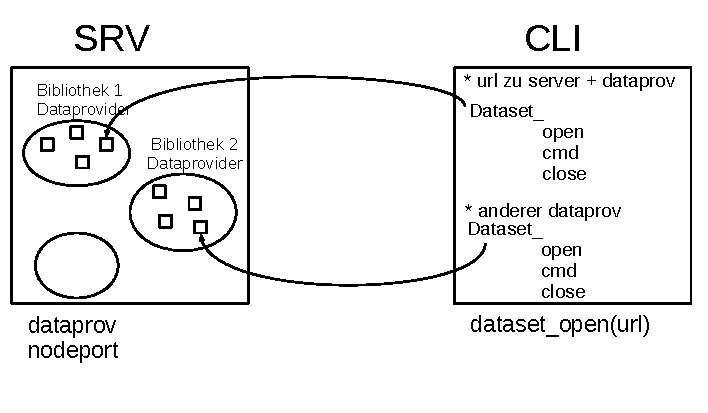
\includegraphics[width=0.7\textwidth]{img/srvcli}
\end{center}


\qline \newpage
%===============================================================================================

\section{Datentypen}
Die scdc\_defs.h beinhaltet vor allem Definitionen von Datentypen.\\
In scdc\_args.h sind weitere Datentypen für den internen Gebrauch.

\subsection{scdcint\_t}\label{scdcint_t}
Bei Rückgabe von scdcint\_t mit Wert \textbf{SCDC\_SUCCESS}(=1LL) oder \textbf{SCDC\_FAILURE}(=0LL)\\
Sonst benutzt zur Übergabe von Integerwerten, dabei können bei Konfigurationen entsprechende Werte durch Defines benannt sein.
\begin{lstlisting}[label={l:scdcint_t}]
typedef long long scdcint_t;
\end{lstlisting}


\subsection{scdc\_nodeport\_t}\label{scdc_nodeport_t}
Handel für einen Nodeport. Rückgabe der Funktion \hyperref[scdc_nodeport_open]{\texttt{scdc\_nodeport\_open()}}
\begin{lstlisting}[label={l:scdc_nodeport_t}]
// in scdc.h :
typedef void *scdc_nodeport_t;
\end{lstlisting}


\subsection{scdc\_dataprov\_t}\label{scdc_dataprov_t}
Als Rückgabe bei \hyperref[scdc_dataprov_open]{\texttt{scdc\_dataprov\_open()}}. Dient als handle für Datenprovider.\\
\begin{lstlisting}[label={l:scdc_dataprov_t}]
typedef void *scdc_dataprov_t;
\end{lstlisting}


\pagebreak
\subsection{scdc\_dataprov\_hook\_t}\label{scdc_dataprov_hook_t}
Die angegeben Funktionen werden beim Datenprovider registriert. Dazu wird eine Variable von diesem Datentyp mit entsprechenden Funktionspointern der Funktion
\hyperref[scdc_dataprov_open]{scdc\_dataprov\_open} als Parameter übergeben.
\begin{minipage}{\textwidth}
\begin{lstlisting}[escapechar={~}, label={l:scdc_dataprov_hook_t}]
typedef struct _scdc_dataprov_hook_t
{
  // in scdc_defs.h :
  /// Datenstruktur nimmt Funktionen entgegen die vom Anwender zu schreiben sind
  scdc_dataprov_hook_open_f                      *open;
  scdc_dataprov_hook_close_f                     *close;
  scdc_dataprov_hook_config_f                    *config;

  scdc_dataprov_hook_dataset_open_f              *dataset_open;
  scdc_dataprov_hook_dataset_close_f             *dataset_close;

  scdc_dataprov_hook_dataset_open_read_state_f   *dataset_open_read_state;
  scdc_dataprov_hook_dataset_close_write_state_f *dataset_close_write_state;

  // Funktion die Kommandos (Berechnungen) auf Daten ausführt
  scdc_dataprov_hook_dataset_cmd_f               *dataset_cmd;

} scdc_dataprov_hook_t;

	/* dataprov_hook Funktionstypen mit FKT-Definition */
	typedef ~\hyperref[scdcint_t]{\texttt{scdcint\_t}}~ scdc_dataprov_hook_config_f( void *dataprov, const char *cmd, const char *param, const char *val, ~\hyperref[scdcint_t]{\texttt{scdcint\_t}}~ val_size, char **result, ~\hyperref[scdcint_t]{\texttt{scdcint\_t}}~ *result_size);
	typedef void *scdc_dataprov_hook_open_f( const char *conf, va_list ap);
	typedef ~\hyperref[scdcint_t]{\texttt{scdcint\_t}}~ scdc_dataprov_hook_close_f( void *dataprov);
	typedef void *scdc_dataprov_hook_dataset_open_f( void *dataprov, const char *path);
	typedef ~\hyperref[scdcint_t]{\texttt{scdcint\_t}}~ scdc_dataprov_hook_dataset_close_f( void *dataprov, void *dataset);
	typedef void *scdc_dataprov_hook_dataset_open_read_state_f( void *dataprov, const char *buf, ~\hyperref[scdcint_t]{\texttt{scdcint\_t}}~ buf_size);
	typedef ~\hyperref[scdcint_t]{\texttt{scdcint\_t}}~ scdc_dataprov_hook_dataset_close_write_state_f( void *dataprov, void *dataset, char *buf, ~\hyperref[scdcint_t]{\texttt{scdcint\_t}}~ buf_size);
	typedef ~\hyperref[scdcint_t]{\texttt{scdcint\_t}}~ scdc_dataprov_hook_dataset_cmd_f( void *dataprov, void *dataset, const char *cmd, const char *params, ~\hyperref[scdc_dataset_input_t]{\texttt{scdc\_dataset\_input\_t}}~ *input, ~\hyperref[scdc_dataset_output_t]{\texttt{scdc\_dataset\_output\_t}}~ *output);

\end{lstlisting}
\end{minipage}

Die \textbf{\texttt{scdc\_dataprov\_hook\_config\_f}} Funktion ist gedacht, um die Konfiguration über eine bestimmte URL aufzurufen und den Datenprovider so während der Laufzeit einzustellen. Beispiele Kapitel \ref{k:hookfunkbsp}.


\subsection{scdc\_dataset\_t}\label{scdc_dataset_t}
Handel auf einen Datensatz. Rückgabe der Funktion \hyperref[scdc_dataset_open]{\texttt{scdc\_dataset\_open()}}\\
\begin{minipage}{\textwidth}
\begin{lstlisting}[escapechar={°}, label={l:scdc_dataset_t}]
// src/lib/scdc/scdc.h:
	typedef struct _scdc_dataset_t *scdc_dataset_t;
    
// src/lib/scdc/scdc.cc:
	struct _scdc_dataset_t	{
	  _scdc_dataset_t()
		:nodeconn(0), dataset(0)
	  {
		buf = new char[DEFAULT_LIBSCDC_BUF_SIZE];
		buf_size = DEFAULT_LIBSCDC_BUF_SIZE;
	  }

	  ~_scdc_dataset_t()
	  {
		delete[] buf;
	  }

	  scdc_nodeconn *nodeconn;
	  scdc_dataset *dataset;
	  char *buf;
	  °\hyperref[scdcint_t]{\texttt{scdcint\_t}}° buf_size;
	};
\end{lstlisting}
\end{minipage}


\subsection{scdc\_dataset\_inout\_intern\_t}\label{scdc_dataset_inout_intern_t}
\begin{minipage}{\textwidth}
\begin{lstlisting}[label={l:scdc_dataset_inout_intern_t}]
// in dataset_inout.h
typedef struct _scdc_dataset_inout_intern_t
{
  scdcint_t alloc_size, type;
  void *buf, *data;

  scdc_dataset_inout_destroy_f *destroy;

} scdc_dataset_inout_intern_t;

// mit Funktionsbeschreibung
typedef void scdc_dataset_inout_destroy_f(scdc_dataset_inout_t *inout);
\end{lstlisting}
\end{minipage}


\pagebreak
\subsection{scdc\_dataset\_input\_t \& scdc\_dataset\_output\_t}\label{scdc_dataset_input_t}\label{scdc_dataset_output_t}\label{scdc_dataset_inout_t}
Mit dieser Struktur wird das Input-Objekt und das Output-Objekt für Datensätze beschrieben. 
Es wird benutzt um die Daten anzugeben, welche zwischen Client und Service Provider übertragen werden. \\
Funktionen dazu in dataset\_inout.h zu finden.\\
Hinweis: \texttt{\_scdc\_dataset\_inout\_intern\_t} und intern\_data bei von Hand befüllen \textbf{ignorieren}.\\
Verwendet von \hyperref[scdc_dataset_cmd]{\texttt{scdc\_dataset\_cmd()}}\\
\begin{minipage}{\textwidth}
\begin{lstlisting}[escapechar={~}, label={l:scdc_dataset_inout_t}]
// in scdc_defs.h :
typedef scdc_dataset_inout_t scdc_dataset_input_t;
typedef scdc_dataset_inout_t scdc_dataset_output_t;

typedef struct _scdc_dataset_inout_t
{
  char format[SCDC_FORMAT_MAX_SIZE];

  scdcint_t buf_size;
  void *buf;

  scdcint_t current_size, total_size;
  char total_size_given;

  scdc_dataset_inout_next_f *next;

  void *data;

  struct ~\hyperref[scdc_dataset_inout_intern_t]{\texttt{\_scdc\_dataset\_inout\_intern\_t}}~ *intern;
  void *intern_data;
  
} scdc_dataset_inout_t;
\end{lstlisting}
\end{minipage}\\
{\begin{minipage}{\textwidth}
\underline{Member}:\\[1ex]
\small
\hspace*{2em}\begin{minipage}{0.8\textwidth}
\begin{description}
\setlength{\itemsep}{-3pt}
\item[- format]: String der das Datenformat beschreibt. Wird mit übertragen und kann beliebig gesetzt werden.
\item[- buf]: Data-Buffer - Die Daten in dem Buffer werden übertragen.
\item[- buf\_size]: Größe des Data-Buffer.
\item[- current\_size]: Größe, bzw. Menge der zur Zeit verfügbaren Daten innerhalb des Data buffers.
\item[- total\_size]: Derzeitig bekannte komplette Menge der Eingabe oder Ausgabe.
\item[- total\_size\_given]: Definiert wie der gegebene Wert total\_size interpretiert wird. Vordefinierte Werte:\\
                              SCDC\_DATASET\_INOUT\_TOTAL\_SIZE\_GIVEN\_EXACT,\\
                              SCDC\_DATASET\_INOUT\_TOTAL\_SIZE\_GIVEN\_AT\_LEAST,\\ 
                              SCDC\_DATASET\_INOUT\_TOTAL\_SIZE\_GIVEN\_AT\_MOST,\\
                              SCDC\_DATASET\_INOUT\_TOTAL\_SIZE\_GIVEN\_NONE.
\item[- next]: Funktionshandel zu einer Funktion, welche den nächsten Teil der Eingabe oder weitere Ausgabedaten liefert. (Sie füllt normalerweise den Buffer mit weiteren Daten, alle Übertragungsdaten komplett sind.)
\item[- data]: Frei nutzbares Daten Feld (z.B. zum Speichern von Zustandsinformationen). Kann benutzt werden um weitere Daten zu hinterlegen, die später benötigt werden. (Speziell Zeiger auf Daten, die die Next-Funktion in den Buffer kopiert, für weitere Übertragung.)
\item[- intern]: Intern von SCDC genutztes Handel. (Nicht für Anwender gedacht, jedoch muss dieses mit der Funktion \hyperref[scdc_dataset_inout_unset]{scdc\_dataset\_output/input\_unset()} auf vordefinierte werte gesetzt werden.)
\item[-  intern\_data]: Frei nutzbares Daten Feld für internen gebrauch.  (Nicht für Anwender nutzbar.)
\end{description}
\end{minipage}
\end{minipage}}

\vspace{2ex}
\pagebreak
\textbf{Funktionsrumpf für Next-Funktion (siehe auch Abs. \ref{scdc_dataset_inout_next_f}):}
\begin{lstlisting}[escapechar={~}, label={l:td_next_fct}]
scdcint_t td_next_fct(struct _scdc_dataset_inout_t *inout)
{
	// Buffer neu Befüllen und alle anderen Werte in inout neu setzen.
	inout->buf          = ...;
	inout->buf_size     = ...;
	inout->current_size = ...;
	// Weiteres ...
	if(<keine Daten>)
		inout->next=NULL; //Wichtig!
		
	return SCDC_SUCCESS;
}
\end{lstlisting}

\begin{minipage}{\textwidth}
Beim Abrufen der Daten aus der Struktur muss die Next-Funktion solange in einer Schleife abgerufen werden bis keine Daten mehr vorhanden sind und 
der Pointer \texttt{inout->next} gleich Null gesetzt ist.
\begin{lstlisting}[escapechar={~}]
if(input->nex != NULL)
{
// Weitere Daten aus input abrufen
input->next(input);
}
else
{ ... /*Alle Daten empfangen*/ }
\end{lstlisting}
\end{minipage}


\subsection{scdc\_dataset\_inout\_next\_f}\label{scdc_dataset_inout_next_f}
Funktionsdescriptor für die next-Funktion.
\begin{lstlisting}[escapechar={°}, label={l:scdc_dataset_inout_next_f}]
// in scdc_defs.h :
typedef °\hyperref[scdcint_t]{\texttt{scdcint\_t}}° scdc_dataset_inout_next_f(struct _scdc_dataset_inout_t *inout);
\end{lstlisting}
Funktion die dazu dient weitere Daten im Buffer bereit zu stellen. Funktion muss vom Anwender geschrieben werden und in der Datenstruktur
\hyperref[scdc_dataset_input_t]{\texttt{scdc\_dataset\_input/output\_t}} unter \textit{next} hinterlegt wird.
Beim Abruf der nächste Daten wird diese Funktion wieder vom Anwender aufgerufen
Funktion der Form (BSP):
\begin{lstlisting}[escapechar={°}]
scdcint_t input_next(scdc_dataset_input_t *input)
{
	// Anpassen der variable scdc_dataset_input_t *input
	// mit neuen Werten
	set_new(input->buf)
	set_correct_values(input)
	
	return SCDC_SUCCESS;
}
\end{lstlisting}

Auslesen: Next-Funktion immer händisch aufrufen und erneut buf auslesen.
Gedacht um Daten zu übertragen die nicht mit einmal im Speicher liegen. 
Zu große Datenmenge oder on-the-fly generierte Daten sind dann so auch übertragbar.





\qline \newpage
%===============================================================================================

\section{Funktionsrümpfe für Hook-Funktionen}\label{k:hookfunkbsp}


\subsection{\textbf{Funktion:} scdc\_dataprov\_hook\_open\_f}\label{scdc_dataprov_hook_open_f}
\begin{lstlisting}[escapechar={~}]
void* hook_dataprov_open(const char *conf, va_list ap)
{
	// initialisierungen allocation von Speicher usw.
	return <..dataprov..>
}
\end{lstlisting}

\underline{Parameter:}
\begin{tabbing}
conf \= $\leftarrow$ conf \= aus> \= ---------------------------------------------------------------------------------- \kill
conf \> $\leftarrow$ conf \> aus> \> \Hhref{scdc_dataprov_open}(const char *base\_path, const char \textbf{*conf}, ...)\\
ap   \> $\leftarrow$ ...  \> aus> \> \Hhref{scdc_dataprov_open}(const char *base\_path, const char *conf, \textbf{...})\\
\end{tabbing}
\underline{Return} <..dataprov..> Wert im Parameter verwendet von:
\begin{tabbing}
dataprov \= $\Rightarrow$ \= ---------------------------------------------------------------------------------- \kill
dataprov \> $\Rightarrow$ \> \Hhref{scdc_dataprov_hook_close_f}( void \textbf{*dataprov})\\
dataprov \> $\Rightarrow$ \> \Hhref{scdc_dataprov_hook_config_f}(void \textbf{*dataprov}, \underline{~~~~} )\\
dataprov \> $\Rightarrow$ \> \Hhref{scdc_dataprov_hook_dataset_open_f}( void \textbf{*dataprov} , \underline{~~~~} );\\
dataprov \> $\Rightarrow$ \> \Hhref{scdc_dataprov_hook_dataset_close_f}( void \textbf{*dataprov} , \underline{~~~~} );\\
dataprov \> $\Rightarrow$ \> \Hhref{scdc_dataprov_hook_dataset_open_read_state_f}( void \textbf{*dataprov} , \underline{~~~~} );\\
dataprov \> $\Rightarrow$ \> \Hhref{scdc_dataprov_hook_dataset_close_write_state_f}( void \textbf{*dataprov} , \underline{~~~~} );\\
dataprov \> $\Rightarrow$ \> \Hhref{scdc_dataprov_hook_dataset_cmd_f}( void \textbf{*dataprov} , \underline{~~~~} );\\
\end{tabbing}

%--------------------------------------------------------------------------------------------------------------------------------------------------

\subsection{\textbf{Funktion:} scdc\_dataprov\_hook\_close\_f}\label{scdc_dataprov_hook_close_f}
\begin{lstlisting}[escapechar={~}]
scdcint_t hook_dataprov_close(void *dataprov)
{
	 // free ...
	return SCDC_SUCCESS;
}
\end{lstlisting}

\underline{Parameter:}
\begin{tabbing}
dataprov \= $\leftarrow$ return <..dataprov..> \= aus> \= ------------------------------------------------------------ \kill
dataprov \> $\leftarrow$ return <..dataprov..> \> aus> \> \Hhref{scdc_dataprov_hook_open_f}( \underline{~~~~} )\\
\end{tabbing}

%--------------------------------------------------------------------------------------------------------------------------------------------------

\subsection{\textbf{Funktion:} scdc\_dataprov\_hook\_config\_f}\label{scdc_dataprov_hook_config_f}
\begin{lstlisting}[escapechar={~}]
scdcint_t hook_dataprov_config(void *dataprov, const char *cmd,
              const char *param, const char *val, scdcint_t val_size, 
                                char **result, scdcint_t *result_size)
{
    return SCDC_SUCCESS;
}
\end{lstlisting}

\underline{Parameter:}
\begin{tabbing}
dataprov \= $\leftarrow$ return <..dataprov..> \= aus> \= ------------------------------------------------------------- \kill
dataprov \> $\leftarrow$ return <..dataprov..> \> aus> \> \Hhref{scdc_dataprov_hook_open_f}( \underline{~~~~} )\\
\end{tabbing}

%--------------------------------------------------------------------------------------------------------------------------------------------------

\subsection{\textbf{Funktion:} scdc\_dataprov\_hook\_dataset\_open\_f}\label{scdc_dataprov_hook_dataset_open_f}
\begin{lstlisting}[escapechar={~}]
void *hook_dataset_open( void *dataprov, const char *path)
{
	// Anlegen des Datenset, Allokation von Speicher usw.
	return <..dataset..>
}
\end{lstlisting}

\underline{Parameter:}
\begin{tabbing}
dataprov \= $\leftarrow$ return <..dataprov..> \= aus> \= --------------------------------------------------------------- \kill
dataprov \> $\leftarrow$ return <..dataprov..> \> aus> \> \Hhref{scdc_dataprov_hook_open_f}( \underline{~~~~} )\\
path \> $\leftarrow$ uri                       \> aus> \> \Hhref{scdc_dataset_open}( (const char \textbf{*uri}, ...) )\\
\end{tabbing}
\underline{Return} <..dataset..> Wert im Parameter verwendet von:
\begin{tabbing}
dataset \= $\Rightarrow$ \= ---------------------------------------------------------------------------------- \kill
dataset \> $\Rightarrow$ \> \Hhref{scdc_dataprov_hook_dataset_close_f}( \underline{~~}, void \textbf{*dataset}, \underline{~~})\\
dataset \> $\Rightarrow$ \> \Hhref{scdc_dataprov_hook_dataset_close_write_state_f}( \underline{~~}, void \textbf{*dataset}, \underline{~~})\\
dataset \> $\Rightarrow$ \> \Hhref{scdc_dataprov_hook_dataset_cmd_f}( \underline{~~}, void \textbf{*dataset}, \underline{~~})\\
\end{tabbing}


%--------------------------------------------------------------------------------------------------------------------------------------------------

\subsection{\textbf{Funktion:} scdc\_dataprov\_hook\_dataset\_close\_f}\label{scdc_dataprov_hook_dataset_close_f}
\begin{lstlisting}[escapechar={~}]
scdcint_t hook_dataset_close( void *dataprov, void *dataset)
{
	 //free ....
	return SCDC_SUCCESS;
}
\end{lstlisting}

\underline{Parameter:}
\begin{tabbing}
dataprov \= $\leftarrow$ return <..dataprov..> \= aus> \= ----------------------------------------------------------------- \kill
dataprov \> $\leftarrow$ return <..dataprov..> \> aus> \> \Hhref{scdc_dataprov_hook_open_f}( \underline{~~~~} )\\
dataset  \> $\leftarrow$ return <..dataset..>  \> aus> \> \Hhref{scdc_dataprov_hook_dataset_open_f}( \underline{~~~~} )\\
\end{tabbing}

%--------------------------------------------------------------------------------------------------------------------------------------------------

\subsection{\textbf{Funktion:} scdc\_dataprov\_hook\_dataset\_open\_read\_state\_f}\label{scdc_dataprov_hook_dataset_open_read_state_f}
\begin{lstlisting}[escapechar={~}]
 // Wie kann Datensatz serialisiert werden, 
 // für komplexe strukturen, wenn nicht angegeben wird 
 // einfach der zeiger zum client geschickt
void *hook_dataset_open_read_state( void *dataprov, const char *buf, scdcint_t, buf_size)
{
	return <..Kennung..>
}
\end{lstlisting}

\underline{Parameter:}
\begin{tabbing}
dataprov \= $\leftarrow$ return <..dataprov..> \= aus> \= -------------------------------------------------------------------- \kill
dataprov \> $\leftarrow$ return <..dataprov..> \> aus> \> \Hhref{scdc_dataprov_hook_open_f}( \underline{~~~~} )\\
\end{tabbing}
%--------------------------------------------------------------------------------------------------------------------------------------------------

\subsection{\textbf{Funktion:} scdc\_dataprov\_hook\_dataset\_close\_write\_state\_f}\label{scdc_dataprov_hook_dataset_close_write_state_f}
\begin{lstlisting}[escapechar={~}]
scdcint_t hook_dataset_close_write_state( void *dataprov, void *dataset, char *buf, scdcint_t buf_size)
{
	// Was Berechnen
	return SCDC_SUCCESS;
}
\end{lstlisting}

\underline{Parameter:}
\begin{tabbing}
dataprov \= $\leftarrow$ return <..dataprov..> \= aus> \= ----------------------------------------------------------------- \kill
dataprov \> $\leftarrow$ return <..dataprov..> \> aus> \> \Hhref{scdc_dataprov_hook_open_f}( \underline{~~~~} )\\
dataset  \> $\leftarrow$ return <..dataset..>  \> aus> \> \Hhref{scdc_dataprov_hook_dataset_open_f}( \underline{~~~~} )\\
\end{tabbing}
%--------------------------------------------------------------------------------------------------------------------------------------------------

\subsection{\textbf{Funktion:} scdc\_dataprov\_hook\_dataset\_cmd\_f}\label{scdc_dataprov_hook_dataset_cmd_f}
\begin{lstlisting}[escapechar={~}]
scdcint_t hook_dataset_cmd(void *dataprov, void *dataset, const char *cmd, const char *params,
                                    scdc_dataset_input_t *input, scdc_dataset_output_t *output)
{
	 // Verarbeitung von Daten
	 // Input und Output über input und output siehe Parameter
	 
	 if(input->nex != NULL)
	 {
	 	// Weitere Daten aus input abrufen
	 	input->next(input);
	 }
	 else
	 { ... // Alle Daten empfangen}
    
	return SCDC_SUCCESS;	
}

\end{lstlisting}

\underline{Parameter:}
\begin{tabbing}
dataprov \= $\leftarrow$ return <..dataprov..>... \= aus> \= ----------------------------------------------------------------- \kill
dataprov \> $\leftarrow$ return <..dataprov..>    \> aus> \> \Hhref{scdc_dataprov_hook_open_f}( \underline{~~~~} )\\
dataset  \> $\leftarrow$ return <..dataset..>     \> aus> \> \Hhref{scdc_dataprov_hook_dataset_open_f}( \underline{~~~~} )\\

cmd      \> $\leftarrow$ cmd                      \> aus> \> \Hhref{scdc_dataset_cmd}( \underline{~~}, const char \textbf{*cmd} ,\underline{~~} )\\
params   \> $\leftarrow$ cmd (String nach \qqq{~})\> aus> \> \Hhref{scdc_dataset_cmd}( \underline{~~}, const char \textbf{*cmd} ,\underline{~~} )\\
input    \> $\leftarrow$ input                    \> aus> \> \Hhref{scdc_dataset_cmd}( \underline{~~}, scdc\_dataset\_input\_t \textbf{*input} )\\
output   \> $\leftarrow$ output                   \> aus> \> \Hhref{scdc_dataset_cmd}( \underline{~~}, scdc\_dataset\_output\_t \textbf{*output} )\\
\end{tabbing}

%--------------------------------------------------------------------------------------------------------------------------------------------------



\qline \newpage
%===============================================================================================

\section{Funktionen}
%Abkürzungen zu hyperefs:
\newcommand{\Header}[1]{\marginpar[none]{ \hyperref[#1]{{H\\[-1em]{\fontsize{4pt}{2pt}\selectfont\hspace*{-3em}\detokenize{#1}}}} }}
\newcommand{\scdcintt}[0]{\hyperref[scdcint_t]{scdcint\_t} }
\newcommand{\scdcdatasett}[0]{\hyperref[scdc_dataset_t]{scdc\_dataset\_t} }
\newcommand{\scdcdatasetinputt}[0]{\hyperref[scdc_dataset_inout_t]{scdc\_dataset\_input\_t} }
\newcommand{\scdcdatasetoutputt}[0]{\hyperref[scdc_dataset_inout_t]{scdc\_dataset\_output\_t} }
\newcommand{\scdcdatasetinoutt}[0]{\hyperref[scdc_dataset_inout_t]{scdc\_dataset\_inout\_t} }
\newcommand{\scdcnodeportt}[0]{\hyperref[scdc_nodeport_t]{scdc\_nodeport\_t} }

\newcommand{\scdcdataprovhookt}[0]{\hyperref[scdc_dataprov_hook_t]{scdc\_dataprov\_hook\_t} }

\sloppy
%------------------------

%\funcdesc{#1=Beschreibung}{#2=\param-parameter}{#3=Rückgabetyp}{#4=beschreibung Rückgabe}
%\param{#1=parametername}{#2=typedefinition}{#3=Beschreibung}

\subsection{SCDC General: init and release}

\subsubsection[scdcint\_t scdc\_init(const char *conf, ...)]{ \scdcintt scdc\_init(const char *conf, ...) }\label{scdc_init}
\Header{scdc.h}
\funcdesc	{Initialisierung der SCDC-Bibliothek mit Konfiguration conf (z. B. SCDC\_INIT\_DEFAULT)}
			{
				\param{conf}{const char * (C) | string (Python)}{Konfiguration für Initialisierung der Bibliothek (Werte=\qqg{SCDC\_INIT\_DEFAULT} (Bisher einzigste) )}
				\param{...}{~}{gibt bisher keine weiteren Argumente}
			}
			{\scdcintt}{SCDC\_SUCCESS oder SCDC\_FAILURE}
%--------------------------------------------------------------------------------------------

\subsubsection[void scdc\_release(void)]{ void scdc\_release(void) }\label{scdc_release}
\Header{scdc.h}
\funcdesc	{Gibt den SCDC-Kontext wieder frei. Finalisierung der SCDC-Bibliothek. Muss am ende aufgerufen werden.}
			{
				\param{--}{void}{ }
			}
			{void}{}
%--------------------------------------------------------------------------------------------

\subsection{SCDC Service: Logging}
\subsubsection[scdcint\_t scdc\_log\_init(const char *conf, ...)]{ \scdcintt scdc\_log\_init(const char *conf, ...) }\label{scdc_log_init}
\Header{scdc.h}
\funcdesc	{Initialisierung der Logging-Funktionen der SCDC-LIB mit Konfiguration conf.}
			{
				\param{conf}{const char * (C) | string (Python)}{Konfiguration (Werte="",??) }
				\param{...}{~}{weitere können sein}
			}
			{\scdcintt}{SCDC\_SUCCESS oder SCDC\_FAILURE}
			
\subsubsection[void scdc\_log\_release(void)]{ void scdc\_log\_release(void) }\label{scdc_log_release}
\Header{scdc.h}
\funcdesc	{Freigabe des Logs und aller für das Logging verwendeten Resourcen}
			{
				\param{--}{void}{ }
			}
			{void}{}
			
%--------------------------------------------------------------------------------------------
% NODEPORTS
%--------------------------------------------------------------------------------------------
\subsection{SCDC Service: node ports (Datenzugriffsmethoden)}
Datenzugriffsmethoden
\begin{itemize}
\item eine Datenzugriffsmethode wird als nodeport bezeichnet
\item standardmäßig ist für jede Komponente ein direkter Zugriff aktiviert
\item weitere Datenzugriffsmethoden können jederzeit eröffnet/geschlossen (open/close) und temporär gestartet/gestoppt (start/stop) werden
\end{itemize}


\subsubsection[scdc\_nodeport\_t scdc\_nodeport\_open(const char *conf, ...)]
              {\scdcnodeportt scdc\_nodeport\_open(const char *conf, ...)}\label{scdc_nodeport_open}
\Header{scdc.h} 
\funcdesc	{Öffnet eine zusätzliche Datenzugriffsmethode mit Konfiguration \textit{conf} auf dem lokalen Knoten. Bereitet den SCDC-Server vor, um ihn dann zu starten und auf einen Port hören zu lassen.
			{\footnotesize
			\begin{itemize}
				\item[-] direct access (conf = \qqq{direct}): access through direct function calls with URI 'scdc://<id>/', first parameter: string specifying the <id> under which the direct access can be performed
				\item[-] UNIX domain socket (conf = \qqq{uds}): access by communication through a local UNIX domain socket with URI 'scdc+uds://<id>/', first parameter: socket name <id> (not implemented, yet)
				\item[-] TCP socket (conf = \qqq{tcp}): access by network communication through a TCP socket with URI 'scdc+tcp://<host>:<port>/', no parameters
				\item[-] message passing interface (conf = \qqq{mpi}): access by communication through stdin with URI 'scdc+mpi://
				\item[-] file stream (conf = \qqq{stream}): access by communication through stdin with URI 'scdc+stream:///', not fully implemented, only used to keep a local service running by waiting for input on stdin
			\end{itemize}
			Variable Parameter ähnlich der \hyperref[scdc_dataprov_open]{Dataprovider}.
			}
			siehe dazu auch Folien \texttt{Datenzugriffsmethoden: nodeport}
            }
			{
				\param{conf}{const char * (C) | string (Python)}{Konfigurationsstring der Type und Parameter des Nodeports festlegt. Werte=(\qqq{direct}, \qqq{uds}, \qqq{tcp}, \qqq{stream}). Nach dem \qqg{:} können noch beliebige Angaben kommen. Bei \qqg{tcp} gibt es bisher nur \qqg{max\_connections}, folglich ist der 2. Parameter eine Intergerzahl der angibt wie viele parallele Verbindungen der Server gleichzeitig annimmt}
				\param{...}{\textit{variabel}}{Zusätzliche angaben, beliebiger art je nachdem was beim ersten Parameter angeben wurde. Z.B: maximale Verbindungsanzahl (int).\\
				           Bisher bekannt:
				           \begin{description}
				           \item{\textbf{\qqq{tcp:max\_connections}} :} INT - Maximale Verbindungen gleichzeitig
				           \end{description}
			               }
			}
			{\scdcnodeportt}{Handel auf neu eröffneten Node/Port. Bei Fehlschlag Rückgabe {\footnotesize SCDC\_NODEPORT\_NULL (C) | False (Python)} }


\subsubsection[void scdc\_nodeport\_close(scdc\_nodeport\_t nodeport)]
               {void scdc\_nodeport\_close(\scdcnodeportt nodeport)}\label{scdc_nodeport_close}
\Header{scdc.h} 
\funcdesc	{Schließen der Datenzugriffsmethode np.}
			{
				\param{nodeport}{\scdcnodeportt}{Handel auf Datenzugriffsmethode}
			}
			{void}{}


\subsubsection[scdcint\_t scdc\_nodeport\_start(scdc\_nodeport\_t nodeport, scdcint\_t mode)]
              {\scdcintt scdc\_nodeport\_start(\scdcnodeportt nodeport, \scdcintt mode)}\label{scdc_nodeport_start}
\Header{scdc.h} 
\funcdesc	{Starten der Datenzugriffsmethode nodeport im Modus mode.\\ 
             Der Modus spezifiziert, ob die Funktion in einer Schleife (LOOP) blockiert bis sie abgebrochen, oder asynchron gestartet wird.}
			{
				\param{nodeport}{\scdcnodeportt}{Handel auf Datenzugriffsmethode}
				\param{mode}{\scdcintt}{Modus (Werte= SCDC\_NODEPORT\_START\_LOOP\_UNTIL\_CANCEL, SCDC\_NODEPORT\_START\_LOOP\_UNTIL\_IDLE (unused),
				              SCDC\_NODEPORT\_START\_ASYNC\_UNTIL\_CANCEL, SCDC\_NODEPORT\_START\_ASYNC\_UNTIL\_IDLE (unused) )}
			}
			{\scdcintt}{Rückgabe ob Erfolgreich. (c: SCDC\_SUCCESS/SCDC\_FAILURE; Py: True/False)}


\subsubsection[scdcint\_t scdc\_nodeport\_stop(scdc\_nodeport\_t nodeport)]
              {\scdcintt scdc\_nodeport\_stop(\scdcnodeportt nodeport)}\label{scdc_nodeport_stop}
\Header{scdc.h} 
\funcdesc	{Stoppen der Datenzugriffsmethode nodeport.}
			{
				\param{nodeport}{\scdcnodeportt}{Handel auf Datenzugriffsmethode}
			}
			{\scdcintt}{Rückgabe ob Erfolgreich. (c: SCDC\_SUCCESS/SCDC\_FAILURE; Py: True/False)}


\subsubsection[scdcint\_t scdc\_nodeport\_cancel(scdc\_nodeport\_t nodeport, scdcint\_t interrupt)]
              {\scdcintt scdc\_nodeport\_cancel(\scdcnodeportt nodeport, \scdcintt interrupt)}\label{scdc_nodeport_cancel}
\Header{scdc.h} 
\funcdesc	{Abbruch einer blockierten Datenzugriffsmethode nodeport.
             Bricht die Datenzugriffsmethode ab, wenn sie im Modus \qqq{SCDC\_NODEPORT\_START\_LOOP\_UNTIL\_CANCEL} gestartet wurde.
             Interrupt = 1 bedeutet \qqg{hartes} abbrechen}
			{
				\param{nodeport}{\scdcnodeportt}{Handel auf Datenzugriffsmethode}
				\param{interrupt}{\scdcintt}{Werte = 1/0}
			}
			{\scdcintt}{Rückgabe ob Erfolgreich. (c: SCDC\_SUCCESS/SCDC\_FAILURE; Py: True/False)}



\subsubsection[const char *scdc\_nodeport\_authority(const char *conf, ...)]
              {const char *scdc\_nodeport\_authority(const char *conf, ...)}\label{scdc_nodeport_authority}
\Header{scdc.h} 
\funcdesc	{Gibt einen \href{https://de.wikipedia.org/wiki/Uniform_Resource_Identifier\#Authority_.28im_Sinne_von_Zust.C3.A4ndigkeit.29}{Authority}-String spezifiziert mit dem Konfigurationsstring conf und den nachfolgenden Parametern (siehe \hyperref[scdc_nodeport_open]{scdc\_nodeport\_open}) für die Datenzugriffsmethode zurück.
			}
			{
				\param{conf}{const char * (C) | string (Python)}{Konfiguration für die Datenzugriffsmethode}
				\param{...}{\textit{variabel}}{ weitere Parameter}
			}
			{const char * (C) | string (Python)}{Authority-String}


\subsubsection[scdcint\_t scdc\_nodeport\_supported(const char *uri, ...)]
              {\scdcintt scdc\_nodeport\_supported(const char *uri, ...)}\label{scdc_nodeport_supported}
\Header{scdc.h} 
\funcdesc	{Abfrage ob Datenzugriffsmethode unterstützt ist ?? }
			{
				\param{uri}{const char * (C) | string (Python)}{URL auf den Ort der Datenzugriffsmethode.??}
				\param{...}{??}{}
			}
			{\scdcintt}{Unterstrützt oder nicht.}

\vfill
%--------------------------------------------------------------------------------------------
% DATAPROVIDER
%--------------------------------------------------------------------------------------------
\subsection{SCDC Service: data providers}

\subsubsection[scdc\_dataprov\_t scdc\_dataprov\_open(const char *base\_path, const char *conf, ...)]
              {scdc\_dataprov\_t scdc\_dataprov\_open(const char *base\_path, const char *conf, ...)}\label{scdc_dataprov_open}
\Header{scdc.h}
\funcdesc	{Öffnet einen zusätzlichen Datenprovider mit der Bezeichnung \textit{path}, welche zugleich den URI-Pfad angibt und der Konfiguration \textit{conf}.
				\begin{itemize}
				\item[-] Konfigurationsstring conf und die nachfolgend Argumente wählen Typ und Parameter des Datenproviders:
				\begin{itemize}
				  \item[-] file system (conf = \qqg{fs}): Zugriff auf das lokale Dateisystem, 1. Parmeter: string Spezifiziert den Wurzelverzeichnis
				  \item[-] generator (conf = \qqg{gen}): Generiert Testdaten, keine Parameter
				  \item[-] MySQL data base (conf = \qqg{mysql}): Zugriff auf eine MySQL Datenbank, 
				           1. Parameter: string \qqg{<dbhost>:<dbuser>:<dbpasswd>:<dbname>} Spezifiziert die Datenbank Anmeldedaten
				  \item[-] hook (conf = \qqg{hook}): Beliebiger Datenprovider konfiguriert mit hook Funktionen, 
				           1. Parameter: Pointer zur Struktur \scdcdataprovhookt (C) | class dataprov\_hook (Python) mit Referenz zu hook Funktionen
				\end{itemize}
				\end{itemize}
				\hspace*{3em} -- Benötigte hook Funktionen: open, close, dataset\_open, dataset\_close,
				                 dataset\_cmd, dataset\_open\_read\_state, dataset\_close\_write\_state
			}
			{
				\param{base\_path}{const char * (C) | string (Python)}{Ort Pfad des Datenproviders (BSP:\qqg{beliebiger})}
				\param{conf}{const char * (C) | string (Python)}{Konfiguration des Handels und der Verbindung des Datenproviders. Der Typ wird durch den Begriff bis zum \qqq{:} angegeben. Danach können entsprechend weitere, teils beliebige String-Fortsetzungen angegeben werden. BSP: \qqg{hook:beliebiger text}.}
				\param{(optional) hookvariable}{\scdcdataprovhookt}{Angabe auf eine Variable welche Handel auf die Hook-Funktionen enthält} 
				\param{...}{~}{Optionale Argumente, die je nach Konfigurationsangabe conf bestimmte Eingaben erfordern.
				              Oder möglich sind auch zusätzliche Argumente, welche beispielsweise an die 
				              \texttt{scdc\_dataprov\_hook\_open\_f *open} Funktion als zweites Argument in dieser, weiter gereicht werden. 
				              Zu finden wären diese anschließend unter dem Parameter \qqg{va\_list ap} 
				              in der \hyperref[scdc_dataprov_hook_open_f]{Dataprov-Hook-Open-Funktion} und  stehen für 
				              weitere individuelle Nutzung dort bereit. }
			}
			{scdc\_dataprov\_t}{Handel des Datenproviders zu dem Verbunden wurde}


\subsubsection[void scdc\_dataprov\_close(scdc\_dataprov\_t dataprov)]
              {void scdc\_dataprov\_close(\hyperref[scdc_dataprov_t]{scdc\_dataprov\_t} dataprov)}\label{scdc_dataprov_close}
\Header{scdc.h}
\funcdesc	{Schließt den Datenprovider des angegebenen Handels}
			{
				\param{dataprov}{\hyperref[scdc_dataprov_t]{scdc\_dataprov\_t} (C)}{Handel des datenproviders}
			}
			{void}{}

%--------------------------------------------------------------------------------------------
% DATASETS
%--------------------------------------------------------------------------------------------
\subsection{SCDC client: data sets}
Datensätze sind vor allem gedacht, um mehrere Kommandos auf Daten auszuführen.

\subsubsection[scdc\_dataset\_t scdc\_dataset\_open(const char *uri, ...)]{\scdcdatasett scdc\_dataset\_open(const char *uri, ...)}\label{scdc_dataset_open}
\Header{scdc.h}
\funcdesc	{Öffnen eines Datensatzes mit URI uri. Prinzip mit den Parametern wie bei \hyperref[scdc_dataprov_open]{Dataprovider} }
			{
				\param{uri}{const char * (C) | string (Python)}{URL des Datensatzes. Beliebiger string}
				\param{...}{const char * (C) | string (Python)}{Können beliebige weitere Parameter mitgegeben werden die dann an die Dataset-Open-Funktion \texttt{scdc\_dataprov\_hook\_dataset\_open\_f *dataset\_open} aus der Struktur \scdcdataprovhookt weiter gegeben wird. Die zusätzlichen Parameter müssen vom Typ Strings sein und zu einem \qqq{\%s} in der uri gehören. Bisher nur \%s und eingefügte Strings unterstützt wie bei printf in c.\\
				 Sonderfall: Ist ein Teil des Pfades der URI \qqg{\%s}, dann wird dieser Teil als String aus dem zusätzlichen Argument gelesen}
			}
			{\scdcdatasett (C)}{Gibt ein Handel auf den neuen Datensatz oderSCDC\_DATASET\_NULL, falls ein Fehler beim Öffnen auftritt, zurück.}


\subsubsection[void scdc\_dataset\_close(scdc\_dataset\_t dataset)]{void scdc\_dataset\_close(\scdcdatasett dataset) }\label{scdc_dataset_close}
\Header{scdc.h}
\funcdesc	{Schließen des Datensatzes dataset}
			{
				\param{dataset}{\scdcdatasett (C)}{Handel auf den Datensatz}
			}
			{void}{}


\subsubsection[scdcint\_t scdc\_dataset\_cmd(ds, cmd, in, out, ...)]
              {\scdcintt scdc\_dataset\_cmd(\scdcdatasett dataset, const char *cmd, \scdcdatasetinputt *input, \scdcdatasetoutputt *output, ...)}\label{scdc_dataset_cmd}
\Header{scdc.h}      
\funcdesc	{Ausführen des Befehls cmd auf dem Datensatz \texttt{dataset} mit Eingabedaten input und Ausgabedaten output.
             Ist \texttt{dataset} gleich SCDC\_DATASET\_NULL wird die URL des Datensatzes vom Anfang des Befehlsstrings cmd gelesen.\\
             Wird das spezielle Handle SCDC\_DATASET\_NULL (C) oder None (Python) verwendet, wird die URL des zu verwendenden Datensatzes
             vom Anfang des Befehls-Strings gelesen.
             D.h. der erste Teil des Kommandos cmd wird als URI für den Datensatz, auf welchem der Rest von cmd als Kommando ausgeführt wird, benutzt. 
             Wird das spezielle Handle DATASET\_NULL verwendet, wird die URL des zu verwendenden Datensatzes vom Anfang des Befehls-Strings gelesen.\\
             Die Instanz dieser URI kann mit einem zusätzlichen Argument spezifiziert werden (see scdc\_dataset\_open)\\
             Bsp: \textnormal{\texttt{scdc\_dataset\_cmd(SCDC\_DATASET\_NULL, \qqg{scdc:/hookdemo CMD PARAM1 PARAM2 PARAM3}, \&input, \&output);}}
            }
			{
				\param{dataset}{\scdcdatasett}{Datensatz auf dem das cmd ausgeführt wird}
				\param{cmd}{const char * (C) | string (Python)}{das Kommando, welches auf den Datensatz angewendet wird}
				\param{input}{\scdcdatasetinputt}{Zeiger auf die Eingabe-Struktur, kann auch Wert \texttt{NULL} übergeben werden}
				\param{output}{\scdcdatasetoutputt}{Zeiger auf die Ausgabe-Struktur, kann auch Wert \texttt{NULL}  übergeben werden}
				\param{...}{~}{??}
			}
			{\scdcintt}{Rückgabe ob Erfolgreich ausgeführt. (c: SCDC\_SUCCESS oder SCDC\_FAILURE; Py: True/False)}


\subsection{SCDC general: dataset input/output}

- Vereinfachtes Anlegen von Eingabe- und Ausgabedatenobjekten\\
- Realisierung oft benutzter Funktionalitäten in Verbindung mit Datenobjekten (z. B. Eingabe aus bzw. Ausgabe in Dateien oder Verzeichnisse)\\
- Datenobjekte können erzeugt/zerstört (create/destroy) und umgeleitet (redirect) werden

\subsubsection[void scdc\_dataset\_input\_print(scdc\_dataset\_input\_t *input)]
              {void scdc\_dataset\_input\_print(\scdcdatasetinputt *input)}\label{scdc_dataset_input_print}
\Header{scdc.h} \Header{dataset_inout.h}
\funcdesc	{Ausgabe des Inhalts (Werte der Struktur-Member) von \texttt{input} auf stdout in einem nerd-lesbaren Format.}
			{
				\param{input}{\scdcdatasetinputt}{Zeiger auf das Dataset-Input-Objekt}
			}
			{void}{}
			
\subsubsection[void scdc\_dataset\_output\_print(scdc\_dataset\_output\_t *output)]
              {void scdc\_dataset\_output\_print(\scdcdatasetoutputt *output)}\label{scdc_dataset_output_print}
\Header{scdc.h} \Header{dataset_inout.h}
\funcdesc	{Ausgabe des Inhalts (Werte der Struktur-Member) von \texttt{output} auf stdout in einem nerd-lesbaren Format.}
			{
				\param{output}{\scdcdatasetoutputt}{Zeiger auf das Dataset-Output-Objekt}
			}
			{void}{}


\subsubsection[void scdc\_dataset\_inout\_unset(scdc\_dataset\_inout\_t *inout)]
              {void scdc\_dataset\_inout\_unset(\scdcdatasetinoutt *inout)}\label{scdc_dataset_inout_unset}
\Header{dataset_inout.h} 
\funcdesc	{Setzt alle Elemente der Struktur \scdcdatasetinoutt auf definierte Nullwerte. Leert das InOut-Objekt.\\
             Diese Funktion sollte nach dem Anlegen einer InOut-Variable benutzt werden, um das Objekt entsprechend zu initialisieren.}
			{
				\param{inout}{\scdcdatasetinoutt}{Zeiger auf das Dataset-Input-Output-Objekt}
			}
			{void}{}
			

\subsubsection[void scdc\_dataset\_input\_unset(scdc\_dataset\_input\_t *input)]
              {void scdc\_dataset\_input\_unset(\scdcdatasetinputt *input)}\label{scdc_dataset_input_unset}
\Header{scdc.h} \Header{dataset_inout.h}
\funcdesc	{Setzt alle Elemente der Struktur \scdcdatasetinputt auf definierte Nullwerte. Leert das input Objekt.\\
             Diese Funktion sollte nach dem Anlegen einer Input-Variable benutzt werden, um das Objekt entsprechend zu initialisieren.}
			{
				\param{input}{\scdcdatasetinoutt}{Zeiger auf das Dataset-Input-Objekt}
			}
			{void}{}


\subsubsection[void scdc\_dataset\_output\_unset(scdc\_dataset\_output\_t *output)]
              {void scdc\_dataset\_output\_unset(\scdcdatasetoutputt *output)}\label{scdc_dataset_output_unset}
\Header{scdc.h} \Header{dataset_inout.h}
\funcdesc	{Setzt alle Elemente der Struktur \scdcdatasetoutputt auf definierte Nullwerte. Leert das Output-Objekt.\\
             Diese Funktion sollte nach dem Anlegen einer Output-Variable benutzt werden, um das Objekt entsprechend zu initialisieren.}
			{
				\param{output}{\scdcdatasetinoutt}{Zeiger auf das Dataset-Output-Objekt}
			}
			{void}{}


\subsubsection[scdc\_dataset\_input\_t *scdc\_dataset\_input\_create(scdc\_dataset\_input\_t *input, const char *conf, ...)]
               {\scdcdatasetinputt *scdc\_dataset\_input\_create(\scdcdatasetinputt *input, const char *conf, ...)}\label{scdc_dataset_input_create}
\Header{scdc.h} \Header{dataset_inout.h}
\funcdesc	{ Eine zusätzliche Funktion , um ein Eingabe-Objekt entsprechend der angegebenen Konfiguration zu erzeugen.
			  Nutzbar für Spezielfälle des Ausgabeobjektes. Zum Beispiel um Daten von einer Datei einzulesen. 
			  Vereinfacht in bestimmten Fällen das Anlegen des Eingabeobjektes \texttt{input}.\\
			  Mit dieser Funktion ist es möglich, die Eingabe von verschiedenen Quellen einzulesen.\\
			  Unterstützte Typen und zusätzliche Parameter:\\[1.5ex]
			  \hspace*{1.8cm}\begin{minipage}[b]{0.9\textwidth}
			  \begin{itemize}
			  \item[-~~~\qqq{none}:]  keine Eingabe
			  \item[-~~\qqq{alloc}:] Alloziert einen Eingabepuffer (ohne Inhalt) von dem die Eingabe gelesen wird. Wird der optionale Parameter \qqq{size} angegeben, dann kann die Puffergröße in der zusätzliche Liste mit variablen Parametern spezifiziert werden.
			  \item[-~\qqq{buffer}:] Liest die Eingabe von einem existierenden Speicherbereich. Der Zeiger auf den Puffer und die Größe des Speicherbereichs werden in einer zusätzliche Liste mit variablen Parametern spezifiziert.
			  \item[-~\qqq{stream}:] Benutzt einen I/O-Stream für die Eingabe. Das zum Zeiger zugehörige Fileobjekt muss in der zusätzliche Liste mit den  variablen Parametern angegeben werden.
			  \item[-~~~\qqq{file}:] Benutzt eine lokale Datei für die Eingabe. Der Dateiname mit Pfad muss in der zusätzliche Liste mit den variablen Parametern angegeben werden.
			  \item[-~~~~~\qqq{fs}:] Benutzt ein lokales Dateisystem (Filesystem vgl. Datei,Ordner,..) für die Eingabe. Der Pfad muss in der zusätzliche Liste mit variablen Parametern angegeben werden.
			  \item[-~\qqq{fslist}:] Liest die Eingabe aus lokalen Dateien und Verzeichnissen, welche hier zuvor in einem String in Form einer Liste angegeben wurden. Der Pfad zu den aufgelisteten Objekten wird in der zusätzliche Liste mit variablen Parametern angegeben.
			  \end{itemize}
			  \end{minipage}
			}
			{
				\param{input}{\scdcdatasetinputt}{Zeiger auf das Dataset-Input-Objekt}
				\param{conf}{const char * (C) | string (Python)}{ Konfiguration - siehe Beschreibung. Ein String, der eine durch Doppelpunkte getrennte Liste mit Angabe des Typs der Eingabe und weitere Parameter, enthält.}
				\param{...}{variabel}{Zusätzliche Liste mit variablen Parametern}
			}
			{\scdcdatasetinputt}{Zeiger auf das Eingabeobjekt oder NULL.}


\subsubsection[void scdc\_dataset\_input\_destroy(scdc\_dataset\_input\_t *input)]
              {void scdc\_dataset\_input\_destroy(\scdcdatasetinputt *input)}\label{scdc_dataset_input_destroy}
\Header{scdc.h} \Header{dataset_inout.h}
\funcdesc	{Zerstört das angegeben Input-Objekt, welches mit \hyperref[scdc_dataset_input_create]{scdc\_dataset\_input\_create()} erstellt wurde.}
			{
				\param{input}{\scdcdatasetinputt}{Zeiger auf das Dataset-Input-Objekt.}
			}
			{void}{}


\subsubsection[scdc\_dataset\_output\_t *scdc\_dataset\_output\_create(scdc\_dataset\_output\_t *output, const char *conf, ...)]
              {\scdcdatasetoutputt *scdc\_dataset\_output\_create(\scdcdatasetoutputt *output, const char *conf, ...)}\label{scdc_dataset_output_create}
\Header{scdc.h} \Header{dataset_inout.h}
\funcdesc	{ Eine zusätzliche Funktion , um ein Output-Objekt entsprechend der angegebenen Konfiguration zu erzeugen.
			  Nutzbar für Spezielfälle des Ausgabeobjektes.\\
			  Mit dieser Funktion ist es möglich für die Ausgabe verschiedene Orte festzulegen. 
			  Zum Beispiel kann die Ausgabe in eine Datei geschrieben werden. 
			  Unterstützte Typen und zusätzliche Parameter:\\[1.5ex]
			  \hspace*{1.8cm}\begin{minipage}[b]{0.9\textwidth}
			  \begin{itemize}
			  \item[-~~~~\qqq{none}:]  keine Ausgabe
			  \item[-~~~\qqq{alloc}:] Alloziert einen Ausgabepuffer. Wird der optionale Parameter \qqq{size} angegeben, dann kann die Puffergröße in der zusätzliche Liste mit variablen Parametern spezifiziert werden.
			  \item[-~~\qqq{buffer}:] Benutzt einen existierenden Speicherbereich für die Ausgabe. Der Zeiger auf den Puffer und die Größe des Speicherbereichs werden in einer zusätzliche Liste mit variablen Parametern spezifiziert.
			  \item[-~~\qqq{stream}:] Benutzt einen I/O-Stream als Ausgabe. Das zum Zeiger zugehörige Fileobjekt muss in der zusätzliche Liste mit variablen Parametern angegeben werden.
			  \item[-~~~~\qqq{file}:] Benutzt eine lokale Datei für die Ausgabe. Der Dateiname muss in der zusätzliche Liste mit variablen Parametern angegeben werden.
			  \item[-~~~~~~\qqq{fs}:] Benutzt ein lokales Dateisystem (Filesystem vgl. Datei,Ordner,..), um die Ausgabe zu speichern. Der Pfad muss in der zusätzliche Liste mit variablen Parametern angegeben werden.
			  \item[-~\qqq{consume}:] Die Ausgabe wird konsumiert ohne weitere Ausgabe. Gleichbedeutend zu \qqq{none}.
			  \end{itemize}
			  \end{minipage}
			}
			{
				\param{output}{\scdcdatasetoutputt}{Zeiger auf das Dataset-Output-Objekt}
				\param{conf}{const char * (C) | string (Python)}{Konfiguration - siehe Beschreibung. Ein String, der eine durch Doppelpunkte getrennte Liste mit Angabe des Typs der Ausgabe und weitere Parameter, enthält.}
				\param{...}{variabel}{Zusätzliche Liste mit variablen Parametern}
			}
			{\scdcdatasetoutputt}{Zeiger auf das Ausgabeobjekt oder NULL.}


\subsubsection[void scdc\_dataset\_output\_destroy(scdc\_dataset\_output\_t *output)]
              {void scdc\_dataset\_output\_destroy(\scdcdatasetoutputt *output)}\label{scdc_dataset_output_destroy}
\Header{scdc.h} \Header{dataset_inout.h}
\funcdesc	{ Zerstört das angegeben Output-Objekt, welches mit \hyperref[scdc_dataset_output_create]{scdc\_dataset\_output\_create()} erstellt wurde.}
			{
				\param{output}{\scdcdatasetoutputt}{zeiger auf das Dataset-Output-Objekt}
			}
			{void}{}

  

\subsubsection[scdcint\_t scdc\_dataset\_input\_redirect(scdc\_dataset\_input\_t *input, const char *conf, ...)]
              {\scdcintt scdc\_dataset\_input\_redirect(\scdcdatasetinputt *input, const char *conf, ...)}\label{scdc_dataset_input_redirect}
\Header{scdc.h} \Header{dataset_inout.h}
\funcdesc	{ Leitet ein existierendes Input-Objekt eines Datensatzes entsprechend der angegebenen Konfiguration \texttt{conf} um.
			  Der Konfigurationsparameter \texttt{conf} beinhaltet eine durch Doppelpunkt getrennte Liste, welche die Umleitung beschreibt.\\
			  \hspace*{1ex}Ist der erste Eintrag der Liste ein \qqq{from}, dann wird der existierende input durch eine neue input Quelle ersetzt.
			  Die anschließende Beschreibung der Quelle kann genau so angegeben werden, 
			  wie bei der Funktion \hyperref[scdc_dataset_input_create]{scdc\_dataset\_input\_create()}.\\
			  \hspace*{1ex}Ist jedoch der erste Eintrag ein \qqq{to} (oder zumindest nicht \qqq{from}), 
			    dann wird der gegebene input über das angegebenen Ziel umgeleitet. 
			  Die anschließende Beschreibung des Ziels kann genau so angegeben werden, 
			  wie bei der Funktion \hyperref[scdc_dataset_output_create]{scdc\_dataset\_output\_create()}
			}
			{
				\param{input}{\scdcdatasetinputt}{Zeiger auf das Dataset-Input-Objekt, welches umgeleitet werden soll.}
				\param{conf}{const char * (C) | string (Python)}{Konfiguration in Form einer durch Doppelpunkt getrennten Liste. Syntax:["from/to:<type>:weiteres"]}
			}
			{\scdcintt}{Rückgabe ob Erfolgreich. (c: SCDC\_SUCCESS oder SCDC\_FAILURE; Py: True/False)}


\subsubsection[scdcint\_t scdc\_dataset\_output\_redirect(scdc\_dataset\_output\_t *output, const char *conf, ...)]
              {\scdcintt scdc\_dataset\_output\_redirect(\scdcdatasetoutputt *output, const char *conf, ...)}\label{scdc_dataset_output_redirect}
\Header{scdc.h} \Header{dataset_inout.h}
\funcdesc	{ Leitet ein existierendes Output-Objekt eines Datensatzes entsprechend der angegebenen Konfiguration \texttt{conf} um.
			  Der Konfigurationsparameter \texttt{conf} beinhaltet eine durch Doppelpunkt getrennte Liste, welche die Umleitung beschreibt.\\
			  \hspace*{1ex}Ist der erste Eintrag der Liste ein \qqq{from}, dann wird der existierende output durch eine neue output Quelle ersetzt.
			  Die anschließende Beschreibung der Quelle kann genau so angegeben werden, 
			  wie bei der Funktion \hyperref[scdc_dataset_input_create]{scdc\_dataset\_input\_create()}.\\
			  \hspace*{1ex}Ist jedoch der erste Eintrag ein \qqq{to} (oder zumindest nicht \qqq{from}), 
			    dann wird der gegebene output zum angegebenen Ziel umgeleitet. 
			  Die anschließende Beschreibung des Ziels kann genau so angegeben werden, 
			  wie bei der Funktion \hyperref[scdc_dataset_output_create]{scdc\_dataset\_output\_create()}.
			}
			{
				\param{output}{\scdcdatasetoutputt}{Zeiger auf das Dataset-Output-Objekt, welches umgeleitet werden soll.}
				\param{conf}{const char * (C) | string (Python)}{Konfiguration in Form einer durch Doppelpunkt getrennten Liste. Syntax:["from/to:<type>:weiteres"]}
				\param{...}{\textit{variabel}}{weitere Paramter, beispielsweise Dateihandel bei \qqq{fs} oder Pointer auf einen Puffer}
			}
			{\scdcintt}{Rückgabe ob Erfolgreich. (c: SCDC\_SUCCESS oder SCDC\_FAILURE; Py: True/False)}


%--------------------------------------------------------------------------------------------
%\subsubsection[]
%              {}\label{}
%\Header{scdc.h} 
%\funcdesc	{Beschreibung}
%			{
%				\param{parametername}{typedefinition}{Beschreibung}
%			}
%			{Rückgabetyp}{Rückgabebeschreibung}
%--------------------------------------------------------------------------------------------



\qline \newpage
%===============================================================================================
\section{Header-Files Funktionszuordnung}

\newcommand{\libtreefkt}[1]{ \hyperref[#1]{ \detokenize{#1}()} }

\begin{center}
\begin{minipage}[t]{0.48\textwidth}
{
\dirtree{%
.1 {\textbf{\large scdc.h}\label{scdc.h}}.
.2 { \libtreefkt{scdc_init} }.
.2 { \libtreefkt{scdc_release} }.
.2 { \libtreefkt{scdc_log_init} }.
.2 { \libtreefkt{scdc_log_release} }.
.2 { \libtreefkt{scdc_dataprov_open} }.
.2 { \libtreefkt{scdc_dataprov_close} }.
.2 { \libtreefkt{scdc_nodeport_open} }.
.2 { \libtreefkt{scdc_nodeport_close} }.
.2 { \libtreefkt{scdc_nodeport_start} }.
.2 { \libtreefkt{scdc_nodeport_stop} }.
.2 { \libtreefkt{scdc_nodeport_cancel} }.
.2 { \libtreefkt{scdc_nodeport_authority} }.
.2 { \libtreefkt{scdc_nodeport_supported} }.
.2 { \libtreefkt{scdc_dataset_open} }.
.2 { \libtreefkt{scdc_dataset_close} }.
.2 { \libtreefkt{scdc_dataset_cmd} }.
.2 { \libtreefkt{scdc_dataset_input_print} }.
.2 { \libtreefkt{scdc_dataset_output_print} }.
.2 { \libtreefkt{scdc_dataset_input_unset} }.
.2 { \libtreefkt{scdc_dataset_output_unset} }.
.2 { \libtreefkt{scdc_dataset_input_create} }.
.2 { \libtreefkt{scdc_dataset_input_destroy} }.
.2 { \libtreefkt{scdc_dataset_output_create} }.
.2 { \libtreefkt{scdc_dataset_output_destroy} }.
.2 { \libtreefkt{scdc_dataset_input_redirect} }.
.2 { \libtreefkt{scdc_dataset_output_redirect} }.
%.2 { \libtreefkt{} }.
}
}
\end{minipage}
\begin{minipage}[t]{0.50\textwidth}
{
\dirtree{%
.1 {\textbf{\large dataset\_inout.h}\label{dataset_inout.h}}.
.2 {\libtreefkt{scdc_dataset_output_printf} }.
.2 {\libtreefkt{scdc_dataset_input_log_cout_print}}.
.2 {\libtreefkt{scdc_dataset_output_log_cout_print}}.
.2 {\libtreefkt{scdc_dataset_input_print} }.
.2 {\libtreefkt{scdc_dataset_output_print} }.
.2 {\libtreefkt{scdc_dataset_inout_unset} }.
.2 {\libtreefkt{scdc_dataset_input_unset} }.
.2 {\libtreefkt{scdc_dataset_output_unset} }.
.2 {\libtreefkt{scdc_dataset_input_create_intern}}.
.2 {\libtreefkt{scdc_dataset_input_create} }.
.2 {\libtreefkt{scdc_dataset_input_destroy} }.
.2 {\libtreefkt{scdc_dataset_output_create_intern}}.
.2 {\libtreefkt{scdc_dataset_output_create} }.
.2 {\libtreefkt{scdc_dataset_output_destroy} }.
.2 {\libtreefkt{scdc_dataset_input_redirect_intern}}.
.2 {\libtreefkt{scdc_dataset_input_redirect} }.
.2 {\libtreefkt{scdc_dataset_output_redirect_intern}}.
.2 {\libtreefkt{scdc_dataset_output_redirect}}.
}
}
\end{minipage}
\end{center}


%\qline \newpage
%%===============================================================================================
%\appendix
%\section{Lib scdc.h}
%\lstinputlisting{../doxygen/scdc.h}
%\pagebreak
%\section{Lib scdc\_defs.h}
%\lstinputlisting{../doxygen/scdc_defs.h}
%\pagebreak
%\section{SRC-API-Beschreibung von 2015}
%\lstinputlisting{appendix/API.txt}


\end{document}
